\newpage
\noindent
\section{Evaluación 5.- Monitoreo de Rendimiento de Servicios}
\subsection{Monitoreo de redimiento SSH}
\noindent
La evaluación de rendimiento SSH lo hacemos por medio de un programa escrito en Python y que utliliza una biblioteca llamada \textbf{paramiko}, que nos brinda herramientas para trabajar con un servidor SSH. \\
Iniciando sesión remotamente con SSH y ejecutando un comando de SSH por medio de la biblioteca podemos conocer el numero de conexiones realizadas al servidor, también podemos conocer el tiempo de conexión una ves que el cliente conectado cierra su conexión, el trafico de entrada y salida, por ultimo, restando el tiempo desde el inicio de sesión menos el tiempo de cierre.

\subsection{Monitoreo de redimiento SMTP}
\noindent
Para evaluar el rendimiento del servicio SMTP, ocupamos las bibliotecas de Python \textbf{smtplib}, \textbf{poplib} y \textbf{impalib} , adicionalmente debemos tener una cuenta de correo existente que tenga acceso a su correo por medio de IMAP4 y POP3 en el servidor SMTP que habilitamos, ya que por medio de un programa en Python, enviaremos un correo con el servidor SMTP, midiendo el tiempo de envió.\\
En el momento que se hace el envió exitoso de SMTP, comenzamos a verificar la bandeja de entrada del correo por medio de POP para para conocer el tiempo que el servicio tarda en recibir el correo, para por ultimo paso borrar los correos creados por esta prueba, haremos el mismo procedimiento con IMAP, de esta manera, conseguimos tanto el tiempo de respuesta de SMTP, IMAP y POP para conocer su rendimiento, si alguno de estos pasos falla el estado del servicio cambiara a "DOWN".

\subsection{Monitoreo de redimiento HTTP}
\noindent
Para conocer el rendimiento de nuestro servidor HTTP, hicimos uso de la biblioteca de Python \textbf{http.client}:
\\
El tiempo de respuesta es calculado enviando una petición GET por un recurso del servidor, en este caso conseguiremos un archivo contenido en el servidor, con el propósito de conocer el tamaño en bytes de la respuesta y cual es el ancho de banda, como el ancho de banda es la cantidad de información o de datos que se puede enviar a través de una conexión de red en un período de tiempo dado, esa cifra la podemos conocer dividiendo el tamaño del archivo conseguido entre el tiempo de respuesta.
\newpage
\noindent
\subsection{Monitoreo de redimiento FTP}
\noindent
Para llevar a cabo el monitoreo del servicio FTP se utilizó el código \textit{ftp-cliente.py} donde se hizo uso de las biblitecas \textbf{urllib.request} y \textbf{ftplib} que nos permite trabajar con archivos de acuerdo con el servidor FTP.\\
Una vez que está iniciado el servidor FTP, el cliente hace una petición de un archivo, solicitando un documento que se encuentra en una ruta especificada y mostrando las credenciales de acceso, el servidor envia el archivo como respuesta, el cliente lo almacena y se termina la conexión, en caso de error, la conexión se cierra de manera automática.
\subsection{Monitoreo de rendimiento DNS}
\noindent
En cuanto al servidor DNS, se monitoraron los valores haciendo uso de la biblioteca \textbf{dns.resolver} que nos permite hacer una conexión al servidor DNS proporcionandole el puerto y la dirección a la que deseamos conectarnos. \\
El cliente inicia la conexión al momento en que se le es asignado una dirección IP o dominio y se define el puerto de conexión, si dichos parámetros son correctos, la conexión al servidor se hace de manera correcta, en caso contrario se muestra un mensaje de error y los parámetros devueltos por el servidor indican que la conexión no se llevó a cabo definiendo el status del servidor como \textit{down}.
\subsection{Resultados Obtenidos}
\noindent
Una vez que se obtuvieron los datos necesarios de cada servidor, se generó un archivo PDF donde se muestran las gráficas generadas y los parámetros de tiempo de respuesta de cada servicio configurado. dicho PDF se muestra a continuación.
\begin{figure}[H]
  \centering
    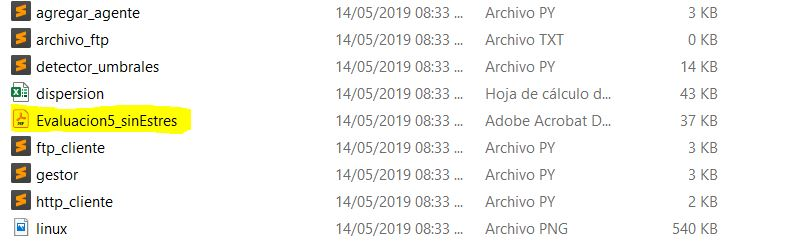
\includegraphics[scale=1]{imagenes/Captura.JPG}
    \caption{PDF Generado}
    \label{fig:http1}
\end{figure}
\begin{figure}[H]
  \centering
    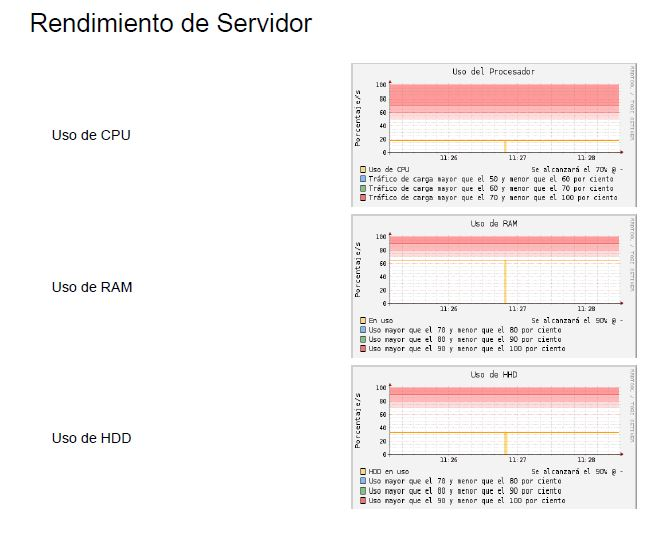
\includegraphics[scale=1]{imagenes/aa1.JPG}
    \caption{Gráficas de Rendimiento del Servidor}
    \label{fig:http1}
\end{figure}
\begin{figure}[H]
  \centering
    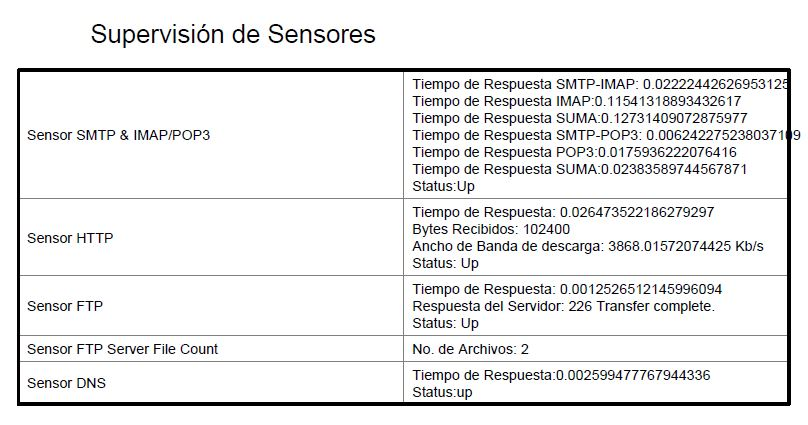
\includegraphics[scale=1]{imagenes/aa2.JPG}
    \caption{Parámetros monitoreados de cada servicio}
    \label{fig:http1}
\end{figure}